%Har gått igenom planeringsrapporten lite noggrannare idag och ser två saker som vi kanske ska borde fånga upp under arbetets gång.

% Under 2 Purpose står det ett upplevelsemål från Young Drive. Bör vi mäta detta upplevelsemål om det stämmer med deltagarnas faktiska upplevelse, d v s ska vi försöka få in det under 3 Research Questions?

% På våra avstämningsmöten borde vi också följa upp dina Research Questions så att kundinteraktionerna och servicedesignmetoden tyligt leder dig framåt mot dessa mål.
%* Reflektioner på vilka designprinciper som bör väljas? (utifrån kundinteraktioner)
%* Reflektioner angående tekniska begränsningar?
%* Reflektioner på processen?

\subsection{Creation of Design Process}
As there was a unfamiliar target group - mostly young Ugandians with little or no experience of smartphones - service design thinking would benefit true understanding of cultural context and in-depth empathy for the end users. Tools and methodology in service design were chosen with the help of Expedition Mondial in Stockholm, who provided education and coaching.

The end result would be a digital artefact (an app), which is not common in service design. While this product could be though of as a service, the tools and methodology would benefit to borrow from Agile methodology and Interaction design. Being a computer expert kind of designer \citep{lowgren} helps being adjusted to agile methodology and interaction design. However, aspiring to be a socio-technical expert, Expedition Mondial are consulted, who are experienced with service design, and are aspiring to be more of computer experts. This led to the joined development of a Digital Service Design method, co-created by the both them and the current author. The result is that the design and development phase in Uganda is an iterative process with the human in focus. The process is built on top of service design process and methodology, while in-line with digital design practices.

%Expedition Mondial helped with a method for creating a MVP of the digital support for the coaches, so that the app was developed from the perspective of the end users and the education and a "learning by doing" mentality.

%The suggested design process was designed with them after a start-up meeting on Skype, and an education day in Stockholm. During that day a crash course in service design was given, then creating a common plan for the future work based on my needs (see Appendix: Original Time Plan \todo{Add reference}). They also recommended service design literature. These were the methods chosen in each iteration.

\subsection{Implementation of Design Process}
There were four iterations. The first iteration follows Service Design, not starting the app development, while the other three follows the new methodology, Digital Service Design. In iteration 1, there is a very broad scope, without digital focus, where iteration 2, 3 and 4 introduces and narrows down the project into a digital solution. In Tororo iteration 1 it was chosen to observe the youth sessions. In Zambia iteration 2 it was decided to observe the coach training. In iteration 3 in Tororo it was chosen to observe the coaches preparing the youth sessions. Figure \ref{fig:methods} is made to assist the reader in the iterations' different focuses.

\begin{figure}[h]
    \centering
    \includegraphics[width=1.0\textwidth]{iterativeprocess2.png}
    \caption{Each of the four iterations had a unique context, app test focus, and research focus. The loops is meant to remind that an iteration consists of three steps before Interactions with the coaches: Insights, Ideation and Trigger material. For more information, see section \ref{digital-service-design} Digital Service Design.}
    \label{fig:methods}
\end{figure}

Expedition Mondial gave support in each iteration, helping with refinements of each iteration as learnings happened along the way, and they were able to educate the current author during the different stages with methodologies whenever necessary, see figure \ref{fig:emSkype}.

\begin{figure}[h]
    \centering
    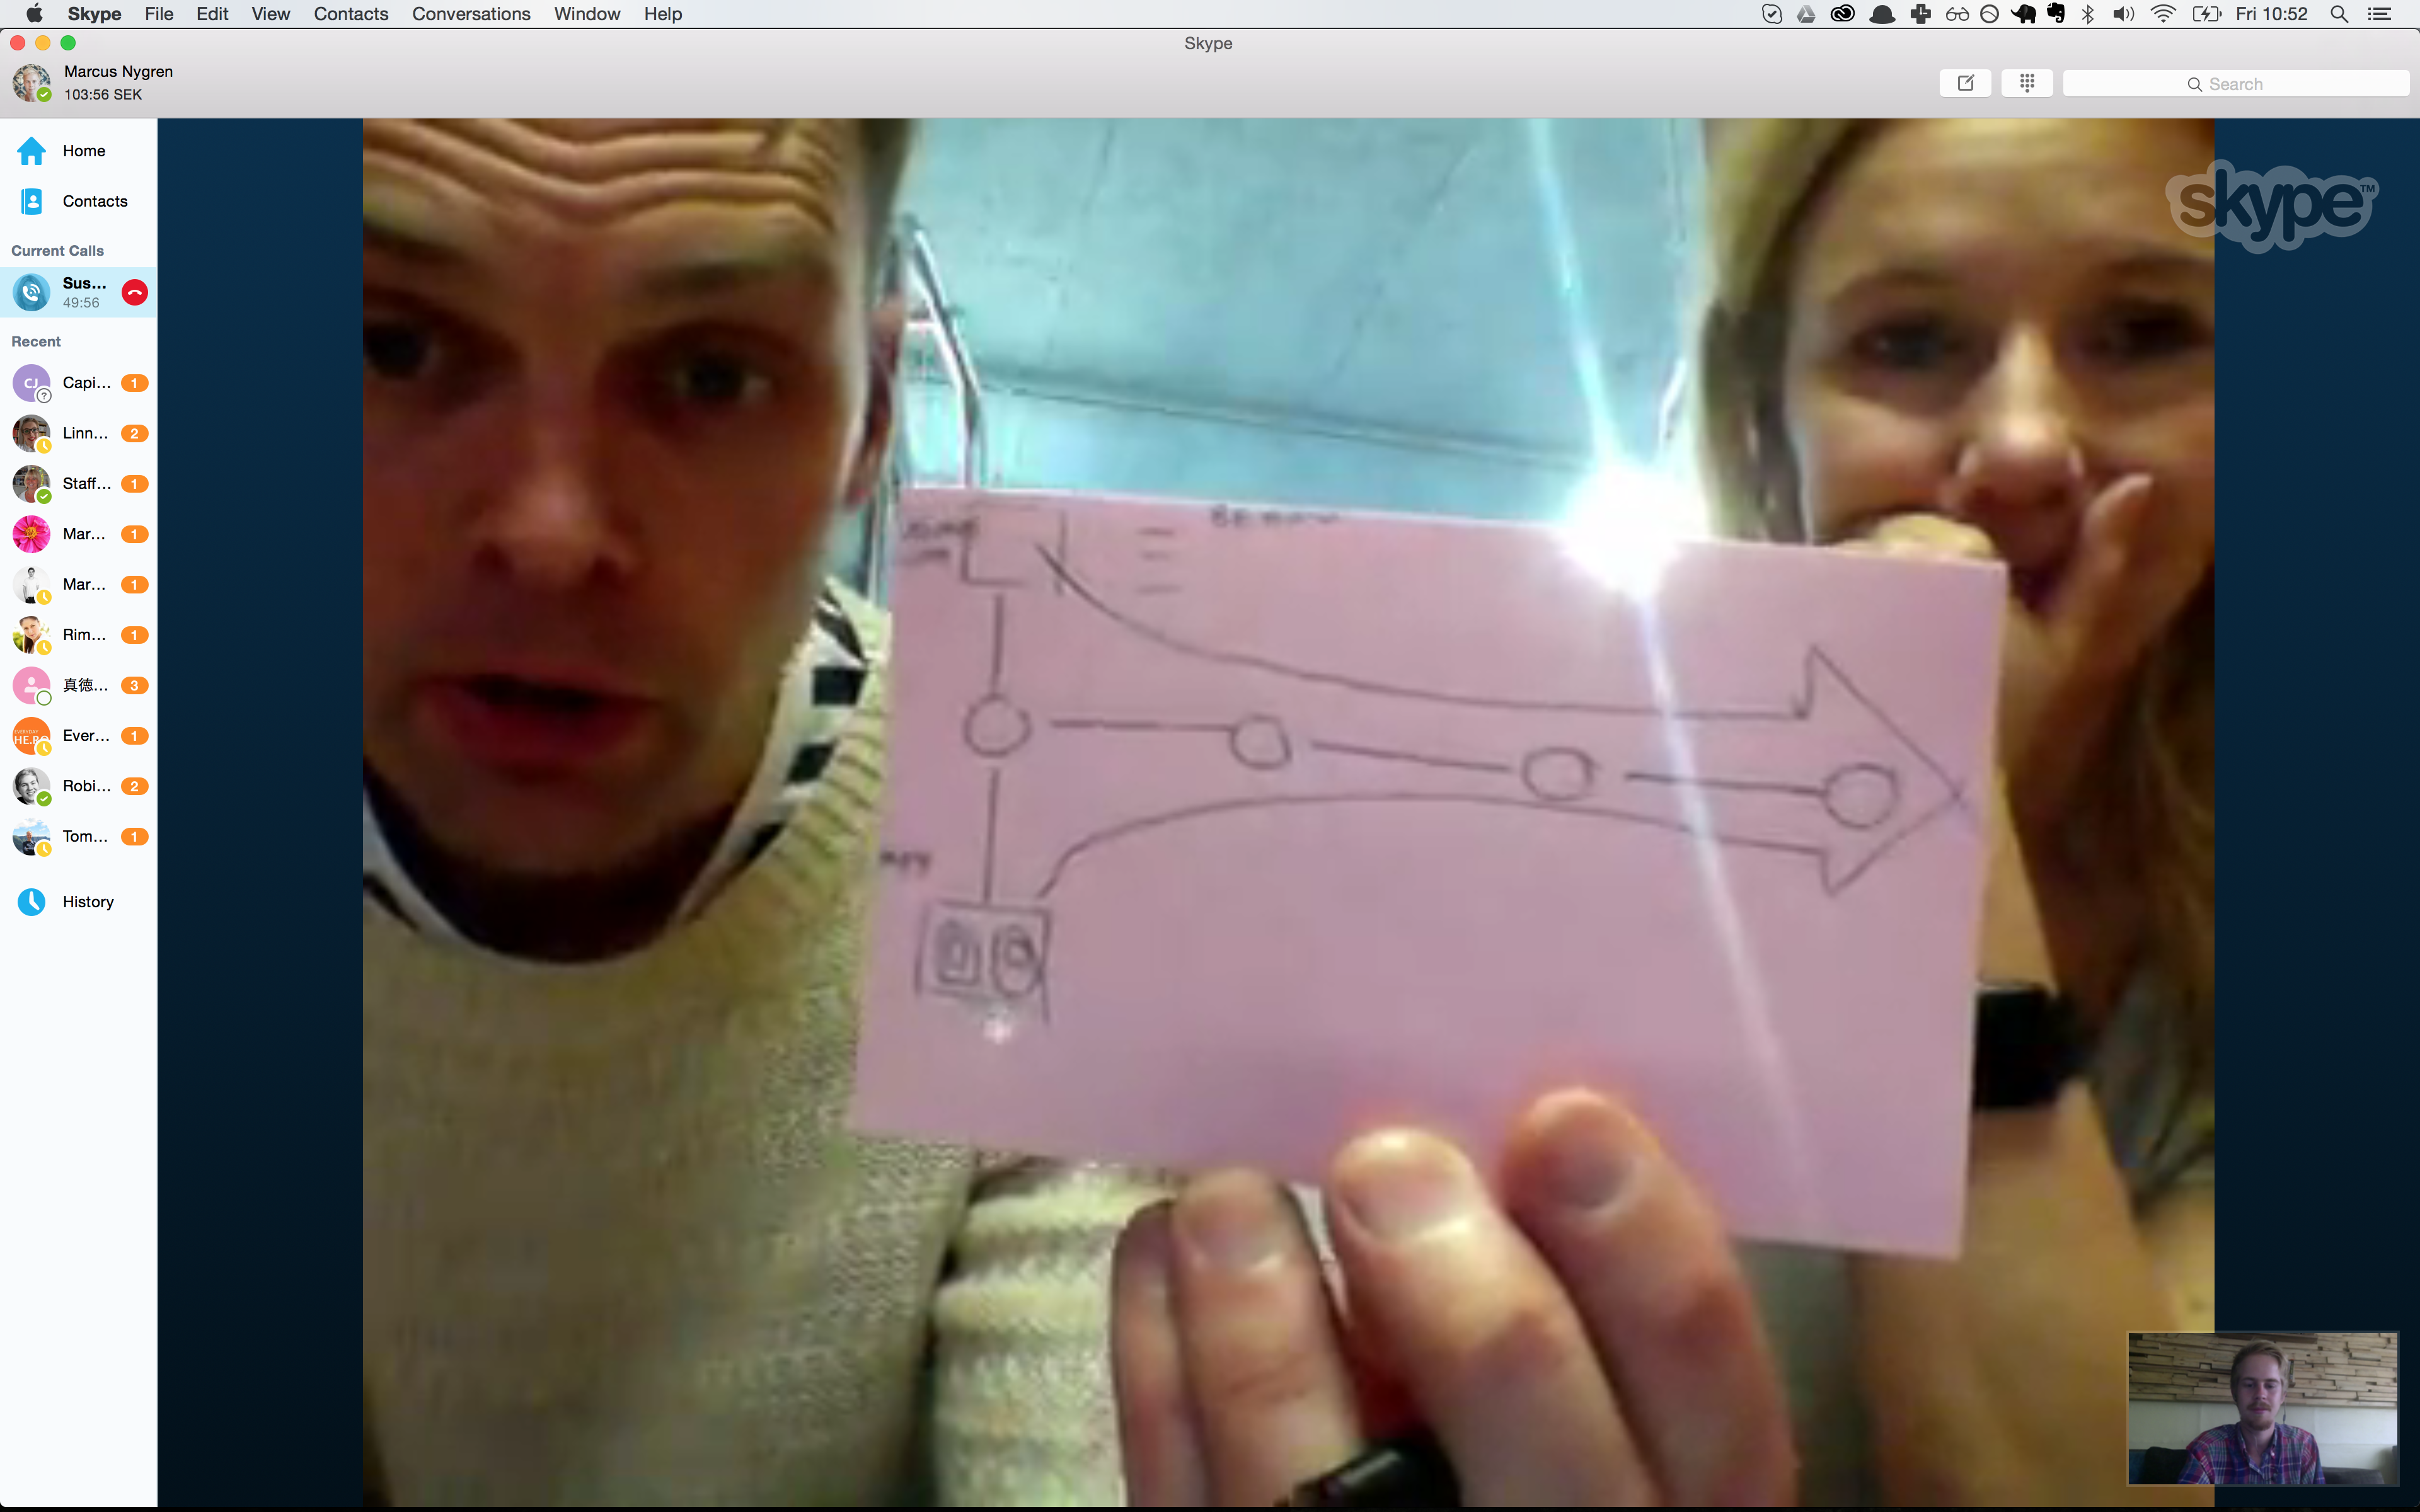
\includegraphics[width=1.0\textwidth]{emSkype.png}
    \caption{In preparation for new situations, like meeting coaches and doing interviews, Nissar and Widmark gave support via Skype videos, sharing service design methodology tips or giving feedback on ideas.}
    \label{fig:emSkype}
\end{figure}
